\documentclass[12pt]{article}

\usepackage{sbc-template}
\usepackage{graphicx,url}
\usepackage{subfig}
\usepackage[utf8]{inputenc}
\usepackage[brazil]{babel}
%\usepackage[latin1]{inputenc}  

     
\sloppy

\title{Análise Exploratória e Visualização de Dados do COVID-19 em Manaus/AM}

\author{David Cardoso Yonekura, Lucas da Silva Lima, Rafael Barbosa de Carvalho}


\address{Universidade do Estado do Amazonas -- Manaus -- Am -- Brazil
  \email{\{dcy.eng17,ldsllm.eng,rbc.eng\}@uea.edu.br}
}

\begin{document} 

\maketitle

\begin{abstract}
    
This technical report describes how the analysis and visualization of COVID-19 data were carried out in the city of Manaus-AM using the dataset provided by the Manaus City Hall. The database went through a filtering process so that certain questions are answered and the visual elaboration of the data, in the form of graphs, was more consistent. In addition, future classification and regression tasks are carried out, such as forecasting the number of people recovered from the disease in the coming months, the locations that will have the highest incidence of cases, among others.
\end{abstract}
     
\begin{resumo} 
  Este relatório técnico descreve como foram realizadas as análises e visualizações de dados de COVID-19 na cidade de Manaus-AM utilizando o dataset disponibilizado pela Prefeitura de Manaus. A base de dados passou por um processo de filtragem para que determinados questionamentos sejam respondidos e a elobaração visual dos dados, na forma de gráficos, fossem mais consistente. Alem disso, futuras tarefas de classificação e regressão sejam realizadas, como por exemplo a previsão na quantidade de pessoas recuperadas da doença nos proximos meses, os locais que terão maior incidencia de casos, entre outros.
\end{resumo}


\section{Introdução}
O cenário de pandemia mundial de COVID-19 \cite{oms} trouxe questões que estão, pouco a pouco, sendo respondidas pela ciência através de diversas técnicas e métodos. Uma estratégia empregada para identificar características da doença como grupos de risco, incidência por idade e letalidade, além da distribuição geográfica e acompanhamento da curva de crescimento de contágio é a utilização de análise exploratória e visualização de dados. O objetivo deste trabalho é identificar e responder questões importantes acerca da manifestação e comportamento do COVID-19 na cidade de Manaus/AM, Brasil, utilizando a linguagem de programação \textbf{Python} e bibliotecas de apoio para sumarizar informações.

\section{Visão geral dos casos confirmados} \label{sec:visaogeral}
O \emph{dataset} utilizado neste trabalho foi disponibilizado pela Prefeitura de Manaus \cite{dataset-covid} e acessado no dia 6 de agosto de 2020. A princípio, foram feitas análises a respeito da quantidade e descrição dos atributos do \emph{dataset}. Com o intuito de visualizar e identificar relações somente com os casos confirmados, optamos por considerar somente estes casos para nossas análises. A quantidade de registros, que anteriormente era de 108351 registros, passou a ser de 36947 registros como mostra a Figura \ref{fig:lineplot}. Foi constatado que o dataset contém 36 atributos que classificam os casos sendo alguns deles: 
Idade, faixa etária, sexo, bairro, classificacao, diabetes, tipos de comorbidades, conclusão, data de notifição, taxa, data de evolução, raça, data dos sintomas, critério, tipo de teste, sintomas, etnia, profissional da saude, srag, evolução. O \emph{dataset} se refere ao período de tempo de 30/01/2020 à 06/08/2020. 

\begin{figure}[ht]
    \centering
    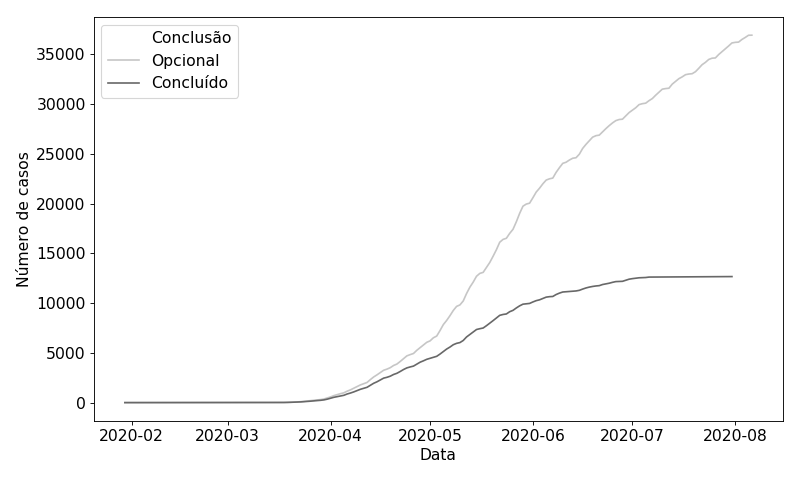
\includegraphics[width=0.84\textwidth]{lineplot_cumulativo.png}
    \caption{Gráfico cumulativo do número de casos, a linha Opcional representa todos os casos confirmados do dataset, e a linha Concluído representa todos os casos que foram concluídos (Recuperado ou Óbito)}
    \label{fig:lineplot}
\end{figure}
Continuando a análise deste projeto, alguns atributos foram removidos para facilitar o direcionamento deste projeto. Os atributos removidos foram: todos os referentes a comorbidades, sintomas, etnia, profissão, datas não referentes a notificação, origem, raça, critério, evolução, tipo de teste, srag e todos os registros com os quais não se tinha informação completa. 


\begin{figure}[ht]
	\centering
	\hfill 
	\subfloat[Boxplot relacionando sexo e idade \label{img:box}]{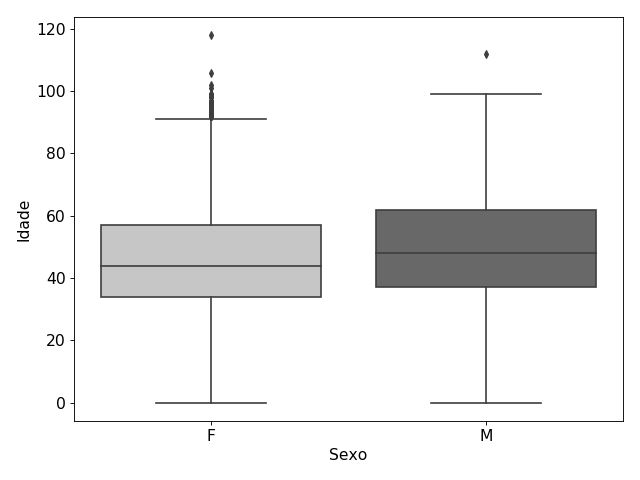
\includegraphics[width=0.4\linewidth]{boxplot_idade.png}} 
	\hfill
	\subfloat[ViolinPlot relacionando sexo, idade e conclusão \label{img:violin}]{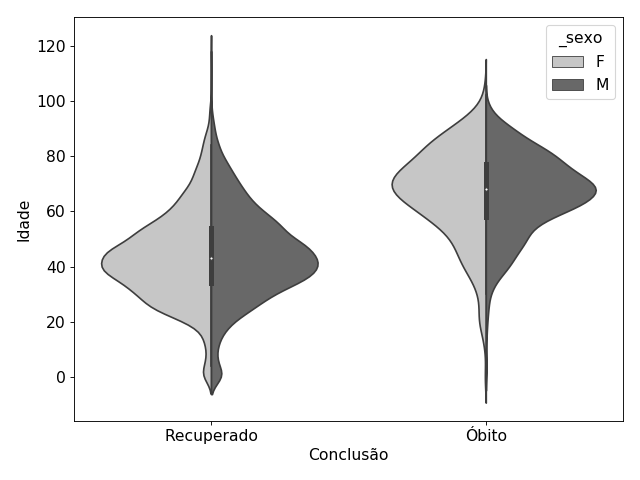
\includegraphics[width=0.4\linewidth]{boxplot_idade_sexo.png}} 
	\hfill
			\caption{Gráficos referentes à distribuição das idades em relação ao sexo e conclusão.}
\end{figure}

Após a filtragem, o dataset continha $12672$ registros e $11$ atributos, com isso tornou-se possível calcular a porcentagem de indivíduos recuperados a qual é $83,917\%$, a quantidade de casos do sexo masculino é de $6367$ e do sexo feminino é de $6305$ mostrando que os homens são marginalmente mais afetados numéricamente, porém, nota-se que a diferença de idade entre os sexos não é tao relevante como ilustrado na Figura \ref{img:box}, inclusive nos indivíduos que se recuperaram ou vieram à óbito como demonstra a Figura \ref{img:violin}. Em seguida, calculando-se a média da idade obtemos o valor de $47,65$ e o desvio padrão de $18,14$.

\begin{figure}[h!]
    \centering
    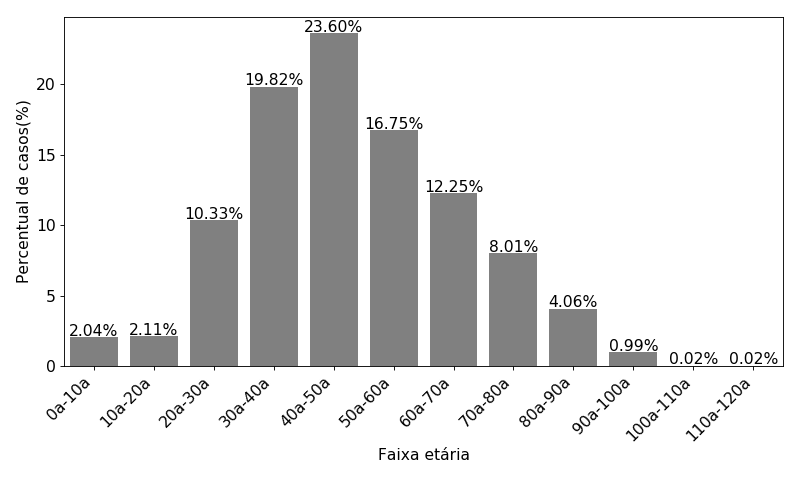
\includegraphics[width=0.8\textwidth]{barplot_faixa.png}
    \caption{Gráfico do percentual de casos em relação a faixa etária.}
    \label{fig:faixa_etaria}
\end{figure}

Após o cálculo da menor e maior idade de todo o registro, obteve-se $0$ anos e $118$ anos como mostrado na Figura \ref{fig:faixa_etaria} indicando que existe a faixa etária a qual essas idades pertencem. Analisando a Figura \ref{fig:scatter} observa-se uma quantidade elevada de casos em indivíduos com 0 anos, é possível que isso seja um erro de entrada, onde casos sem idade definidas foram considerados como 0, outros fatores podem contribuir para essa distribuição concentrada em 40 anos como a distribuição populacional, maior frequência de testes em população de risco e se o indivídiuo faz parte da classe trabalhadora.


\begin{figure}[h!]
    \centering
    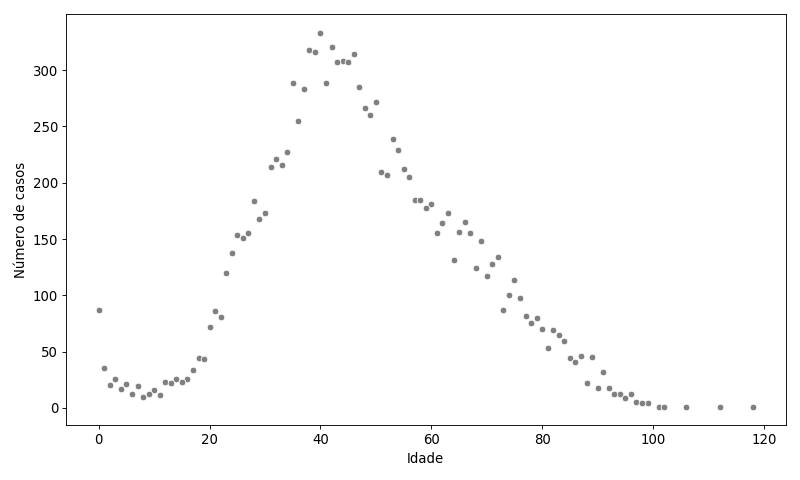
\includegraphics[width=0.7\textwidth]{scatterplot_idade.png}
    \caption{Scatterplot da Idade versus Número de casos }
    \label{fig:scatter}
\end{figure}



No tocante aos bairros, o bairro com a maior incidência de casos é a Cidade Nova, como mostrado na figura \ref{fig:top10_bairros}. Além disso, nota-se que este bairro também teve a maior incidência de casos recuperados. Sendo assim, os três bairros com a maior quantidade de casos recuperados são: Cidade Nova 720, Flores com 438 e Alvorada com 430 casos recuperados.


\begin{figure}[h!]
    \centering
    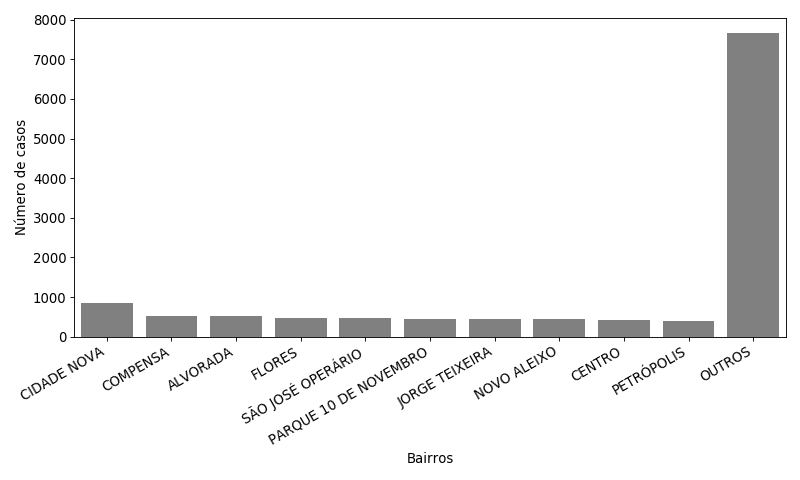
\includegraphics[width=0.8\textwidth]{top10_bairros.png}
    \caption{Gráfico ilustrando a quantidade de todos os casos nos top-10 bairros}
    \label{fig:top10_bairros}
\end{figure}






Seguindo com os tipos de testes realizados, foi necessário repor o atributo de tipo de teste que havia sido filtrado anteriormente para podermos inferir que maior parte dos testes é referente ao Teste Rápido - Anticorpo, representando mais da metade dos testes realizados. Em seguida tal atributo foi filtrado novamente.
\begin{table}[hbt!]
\centering
\caption{Tipos de teste realizados nos casos confirmados de COVID-19.}
\begin{tabular}{|l|c|c|}
	\hline
	Tipo de teste & Quantidade & Percentual\\
	\hline
    Teste Rápido - Anticorpo & 3602 & 57.9659\\
    \hline
    RT-PCR                   & 1501 & 24.1551\\
    \hline
    Teste Rápido - Antígeno  & 1101 & 17.7180\\
    \hline
    ELISA IgM                & 6     & 0.0965\\
    \hline                   
    ECLIA IgG                & 4     & 0.0643\\

	\hline

\end{tabular}
\end{table}

A taxa de letalidade tem, aproximadamente, o valor de $0.16$ e foi calculada utilizando a seguinte equação:

\begin{equation}
L=\frac{Óbitos}{TotalDeCasos}  
\end{equation}

Agrupamos então os casos confirmados por idade e através do método de Correlação de Pearson (Equação \ref{eqn:corr}), que é um grau de relação entre duas variáveis quantitativas que exprime o grau de correlação através de valores situados entre -1 e 1 \cite{pearson}, inferimos o valor de relação de $-0.179869$. Este valor denota uma correlação fraca entre as variáveis, sendo que um valor de magnititude pŕoximo de 1 implica numa alta correlação \cite{atoumscaled}.

\begin{equation}
    \frac{cov(X,Y)}{\sqrt{var(X)\cdot var(Y)}}
    \label{eqn:corr}
\end{equation}


\section{Aplicações}

Um dos possíveis usos dessa base de dados seria determinar se um indivíduo está infectado levando em conta seus sintomas, localização, idade, comorbidades. 

Os sintomas são interessantes visto que boa parte dos casos de COVID-19 apresentam febre, tosse seca e dificuldade respiratória, sendo o último incomum em doenças como a febre e gripe, a localização é útil pois existem áreas com maior incidência de casos, comorbidades e idades que podem afetar o sistema imunológico, facilitando o contagio. O atributo-alvo seria se o caso foi confirmado ou não, configurando uma tarefa de classificação binária, possibilitando o uso de métricas como acurácia, precisão, revocação, curvas ROC e outras métricas relacionadas a erros tipo 1 e 2. 

Por se tratar de uma tarefa relacionada à Medicina, uma validação mais robusta seria necessária, então uma validação cruzada seria o recomendado, dado a quantidade de entradas (100K) uma validação \emph{leave-one-out} poderia ser computacionalmente inviável. Essa classificação não seria usada como um diagnóstico e sim como uma recomendação para procurar ajuda ou manter o isolamento.

\begin{figure}[ht]
    \centering
    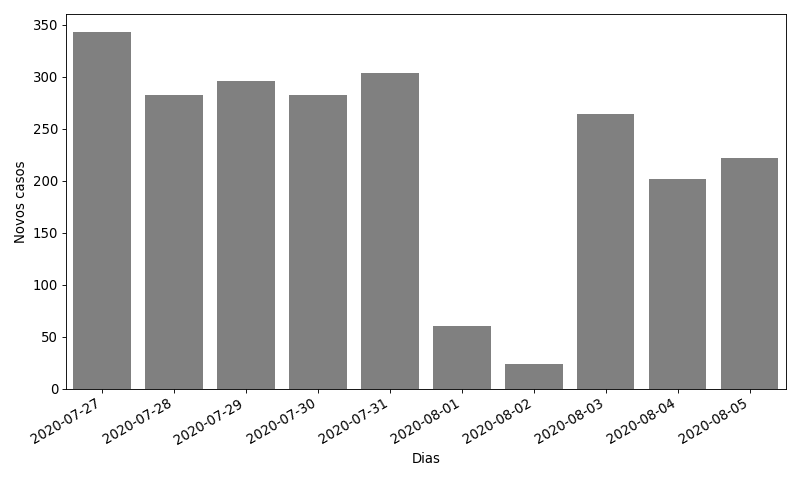
\includegraphics[width=0.7\textwidth]{casos_10_dias.png}
    \caption{Quantidade de novos casos no período dos últimos 10 dias}
    \label{fig:casos_10_dias}
\end{figure}

Outra aplicação seria um modelo para a previsão do número de novos casos, visto que é possível gerar uma série temporal a partir da base de dados como mostra a Figura \ref{fig:casos_10_dias}, onde temos a quantidade de novos casos de um determinado dia. Para aferir o desempenho desse modelo, utiliza-se métricas comuns de regressão como média do erro quadrático ou média do erro absoluto, Além disso, uma validação cruzada própria de séries temporais, na qual a partição de treino sempre engloba os dados mais antigos, e a de validação é adjacente à partição de treino. 


Uma possível aplicação não-supervisionada seria a detecção de anomalias nas mortes por COVID-19. Podemos considerar como anomalia quando uma pessoa saudável ou fora do grupo de risco vem a óbito, o sistema poderia detectar esses casos e uma análise mais profunda poderia ser feita em relação à esses casos específicos, seja averiguar o histórico médico ou contato com a família em busca de outros fatores que poderiam agravar um caso. 

A detecção poderia ser feita utilizando um autoencoder, também vale ressaltar que mesmo usando o rótulo de conclusão para definir quais casos representavam óbitos, a tarefa ainda é não-supervisionado, visto que não temos o rótulo dizendo se um caso é uma anomalia ou não.



\bibliographystyle{sbc}
\bibliography{sbc-template}

\end{document}
